\documentclass[12pt]{beamer}

\setbeamerfont{block body alerted}{size=\small}

\usetheme{Madrid}
\useoutertheme{shadow}

\usepackage{amsfonts}
\usepackage{hyperref}
\usepackage[super,comma,numbers]{natbib}
\renewcommand{\bibnumfmt}[1]{[#1]}
\bibliographystyle{apsrev4-1}

\title[Subordinated Poisson processes for modelling]{Local time subordinating Poisson processes to model semi-permeable membranes}
\author[Hathcock group]{A. Brown | Hathcock group}
\date{January 7, 2026}

\newcommand{\abs}[1]{\left| #1 \right|} % | |
\newcommand{\avg}[1]{\left\langle #1 \right\rangle} % < >
\DeclareMathOperator{\sign}{sgn}

\begin{document}

\maketitle

\begin{frame}{Coarse-graining}
    \begin{figure}
        \centering
        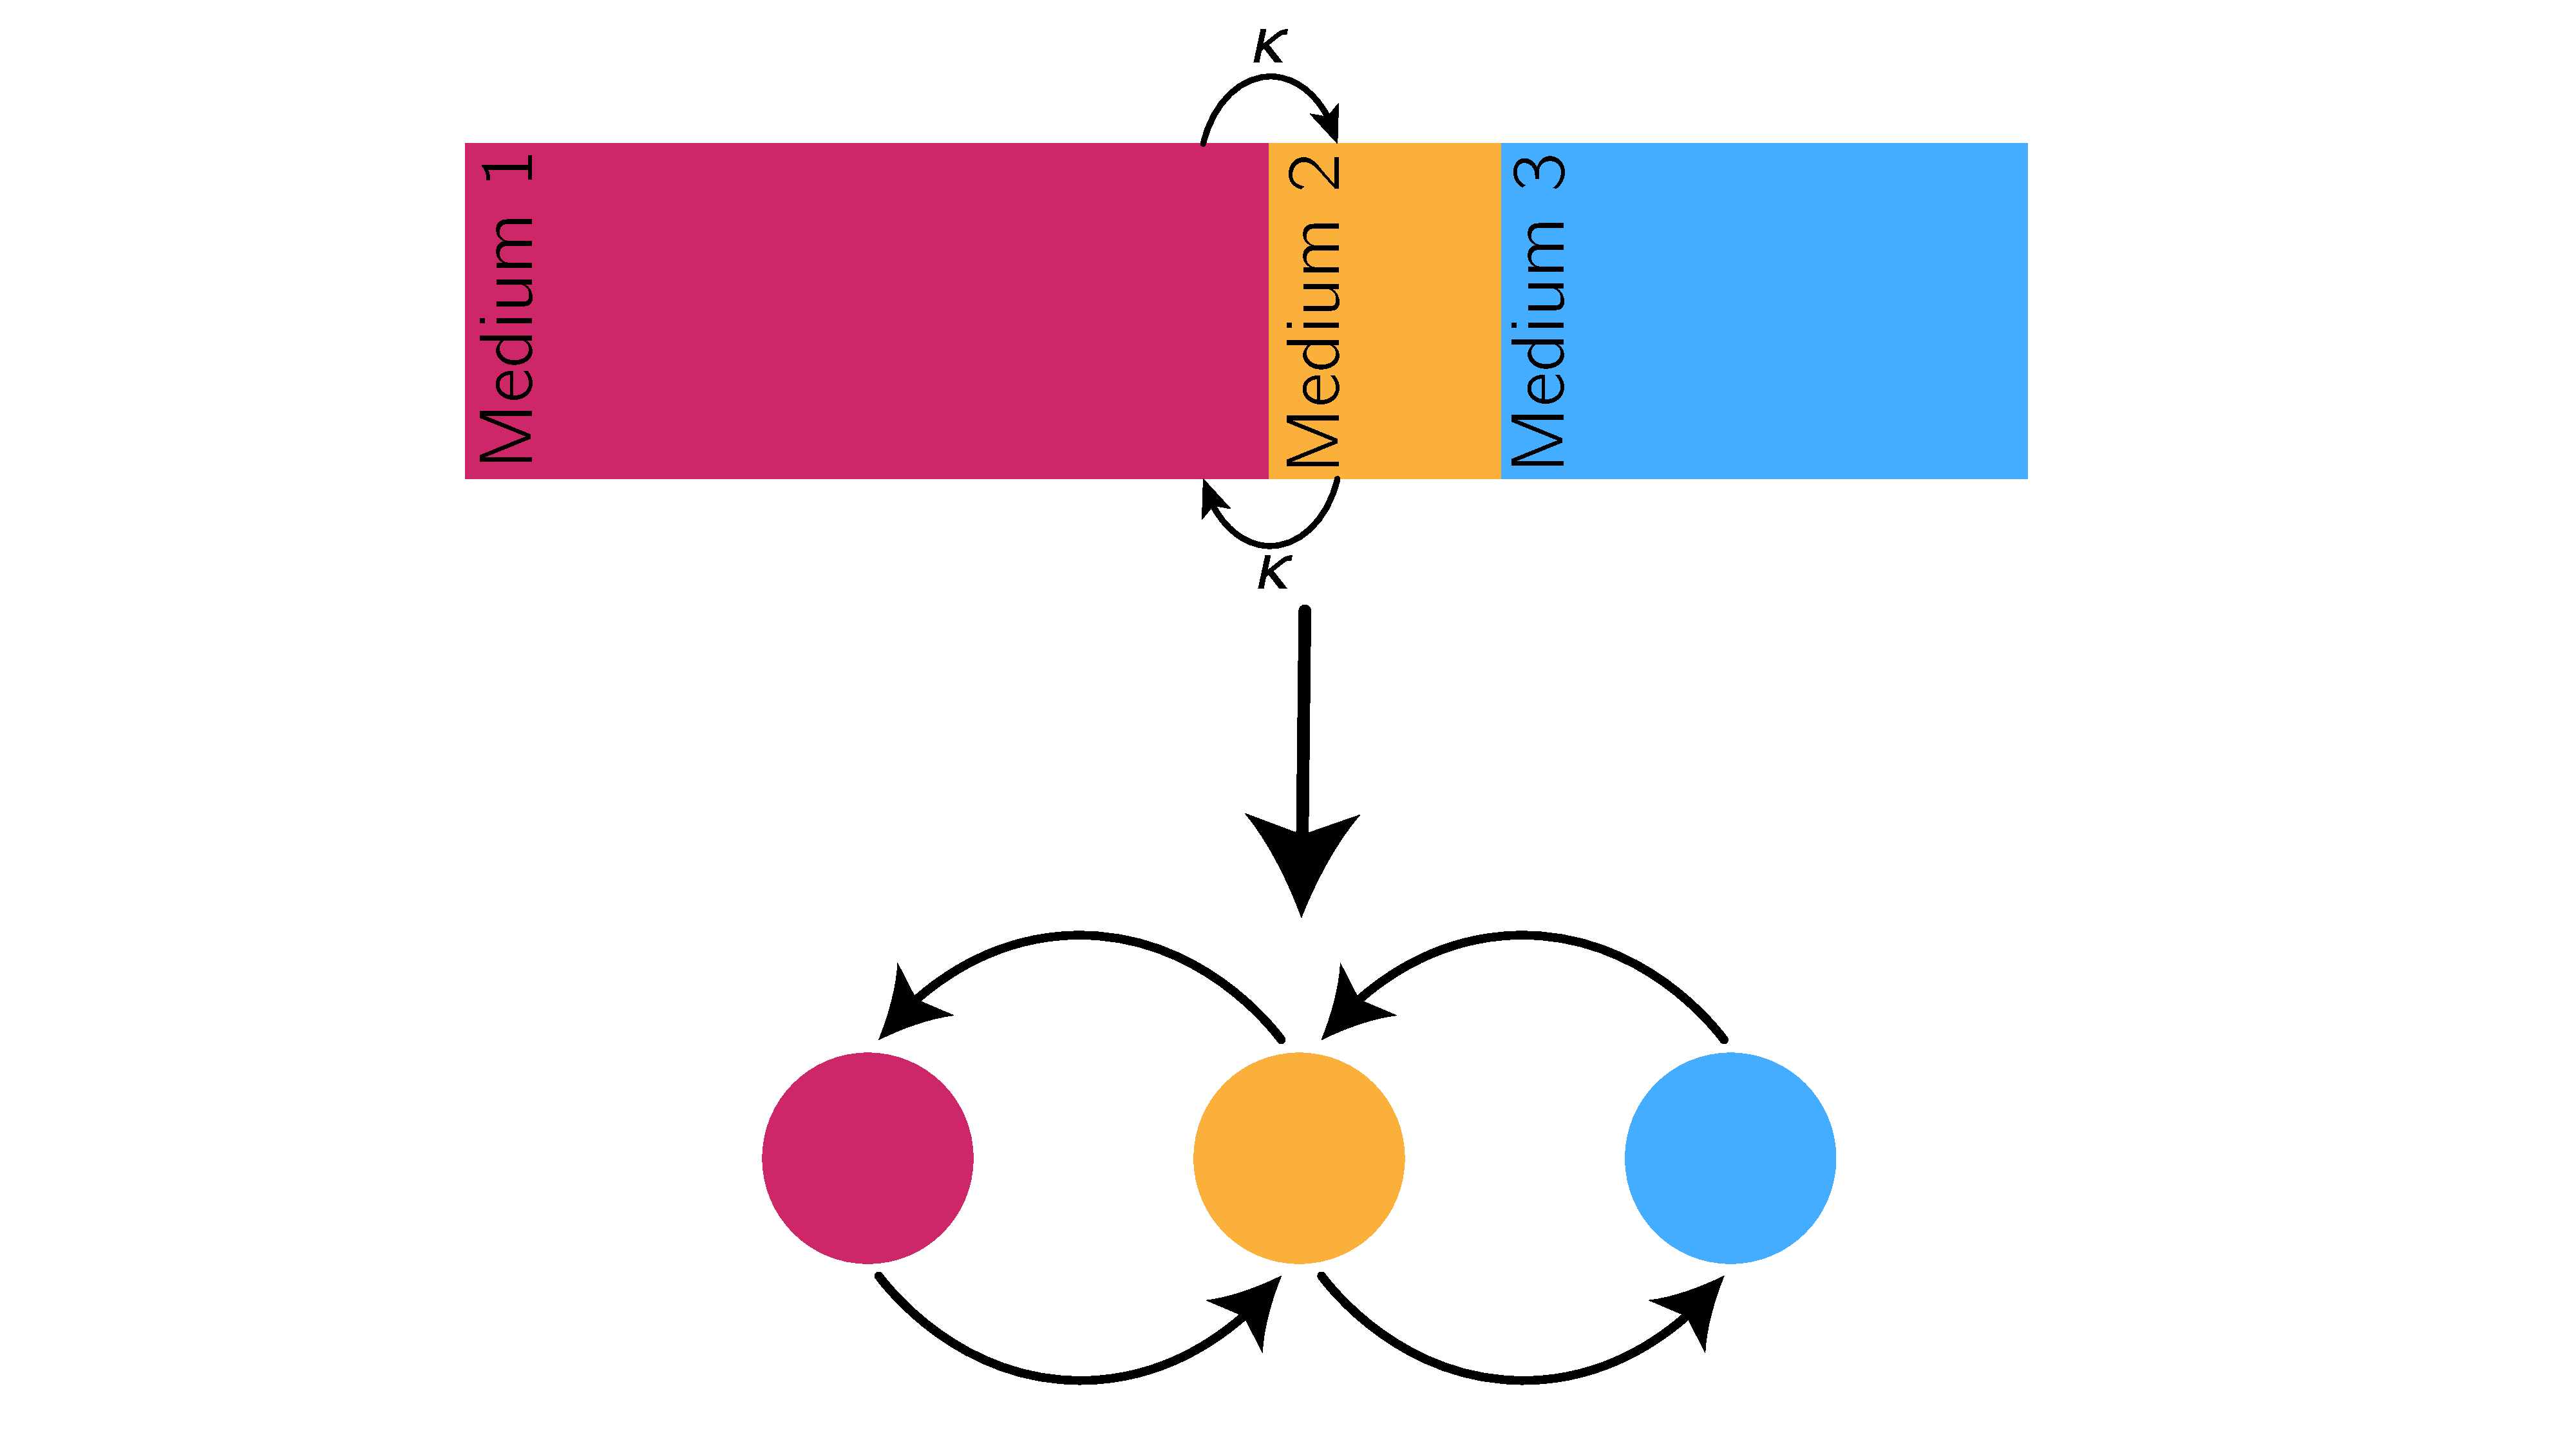
\includegraphics[width=0.7\textwidth]{figures/domain-cg-model.pdf}
    \end{figure}
\end{frame}

\begin{frame}{Local time}
    \begin{itemize}
        \item Let $X_t$ denote a stochastic process on a state space $S \subseteq \mathbb{R}^d$.
        For a point $y \in S$, we define the \textbf{local time} process as
        {%
            \setlength{\belowdisplayskip}{4pt}
            \setlength{\belowdisplayshortskip}{0pt}
            \begin{equation} \label{eq:point-local}
                L_t^y = \int_0^t \delta \left( X_s - y \right) \, d [X_s]
            \end{equation}
        }
        \begin{itemize}
            \item If $X_t$ is a real-valued diffusion, $dX_t = \mu (X, t) \, dt + \sigma (X, t) \, dW_t$, 
            then the quadratic variation is $[X_t] = \int_0^t \sigma^2 (X_s, s) \, ds$ and so $d [X_t] = \sigma^2 (X_t, t) \, dt$.
            Local time thus has units [length]$^{n+1}$ where $n < d$ is the dimension of the (local) manifold
            % see derivation at https://math.stackexchange.com/questions/893025/quadratic-variation-of-diffusion-process-and-geometric-brownian-motion
        \end{itemize}
        \pause
        \item Can reframe our problem as follows:
        A particle moves in a confining domain.
        When near the domain boundary, it is transported through to another domain,
        in a manner dependent upon the ``number of attempts'' to cross it (i.e., local time)~\cite{PhysRevLett.125.078102}
    \end{itemize}
\end{frame}

\begin{frame}{Poisson point processes}
    \begin{itemize}
        \item Choose $\Omega$ to be a domain with a smooth boundary $\partial \Omega$.
        The boundary local time is naturally defined as
        {%
            \setlength{\belowdisplayskip}{0pt}
            \setlength{\belowdisplayshortskip}{0pt}
            \begin{equation} \label{eq:boundary-local}
                L_t^{\partial S} = \int_{\partial \Omega} L_t^x \, d^{d-1} x
            \end{equation}
        }
        \pause
        \item The crossing process of a semi-permeable membrane located at $\partial \Omega$
        can be represented by a Poisson point process 
        subordinated by the boundary local time $\ell_t := L_t^{\partial \Omega}$,~\cite{PhysRevResearch.7.013097}
        \begin{equation} \label{eq:poisson-process}
            \mathbb{P} (N (\ell) = n) = \frac{(q \ell)^n}{n!} e^{- q \ell},
        \end{equation}
        where $q = \kappa / D$ with $\kappa$ the permeability of the membrane and $D$ the (bulk) diffusivity~\cite{PhysRevLett.125.078102}
    \end{itemize}
\end{frame}

\begin{frame}{The Skorokhod equation}
    \begin{itemize}
        \item For a single domain $\Omega \subseteq \mathbb{R}^n$, whereby after reaction, 
        the particle is absorbed by the boundary, the motion is described by the Skorokhod equation~\cite{doi:10.1137/1106035,PhysRevLett.125.078102},
        \begin{equation}\label{eq:skorokhod}
            d X_t = \hat{n} (X) \, d \ell_t + \sqrt{2 D} \, d W_t,
        \end{equation}
        where $\hat{n}$ is the unit normal vector (of fixed orientation) to the boundary $\partial \Omega$
        \pause
        \item Naturally extended to include motion after surface reaction by inverting the direction of the boundary~\cite{PhysRevResearch.7.013097}
        {%
            \setlength{\belowdisplayskip}{0pt}
            \setlength{\belowdisplayshortskip}{0pt}
            \begin{equation}\label{eq:extended-skorokhod}
                d X_t = (-1)^{N (\ell_t)} \hat{n} (X) \, d \ell_t + \sqrt{2 D} \, d W_t,
            \end{equation}
        }
        \pause
        \begin{itemize}
            \item A further extension is to promote the noise to be multiplicative with the boundary separating the media,
            \begin{equation*}
                D(X) = D_1 \mathbb{I}_{\Omega} (X) + D_2 \mathbb{I}_{\mathbb{R}^d \setminus \Omega} (X)
            \end{equation*}
        \end{itemize}
    \end{itemize}
\end{frame}

\begin{frame}
    \begin{itemize}
        \item We now wish to validate that Eq.~\eqref{eq:extended-skorokhod} with multiplicative noise correctly recapilates the PDE form we found previously
        \pause
        \item Following KG 2025~\cite{PhysRevResearch.7.013097}, we make use of
        \begin{alertblock}{The forward Feynman-Kac equation}
            Let $L^* = \mu \partial + \frac{1}{2} \sigma \partial^2$ denote the (adjoint) diffusion generator and
            $d X_t = b (X_t, t) dt + \sigma (X_t, t) d W_t$ its corresponding diffusion process.
            Given the conditional expection of a test function $\phi$ can be written
            \begin{equation}
                \int_\Omega \phi (y) q (y, t \mid x_0) \, dy 
                = \mathbb{E}_{x_0} \left[ \exp{\left( - \int_0^t V (X_s, s) ds \right)} \phi (X_t) \right]
            \end{equation}
            for a potential function $V$, then the (backwards-time) density $q$ satisfies
            \begin{equation}
                \partial_t q (x,t \mid x_0) = (L q) (x,t \mid x_0) - V (x, t) q (x,t \mid x_0)
            \end{equation}
            with $q (x,t \mid x_0) = \delta (x - x_0)$ and appropriate boundary conditions on $\partial \Omega$.
        \end{alertblock}
    \end{itemize}
\end{frame}

\begin{frame}{Application of the Feynman-Kac equation}
    \begin{itemize}
        \item In the ``extended'' Skorokhod equation (ESE), need to consider three processes: $N_t$, $\ell_t$ and $W_t$
        \pause
        \item Probability of $n$ crossings is cond. independent from RBM $Z_t$,
        \begin{equation} \label{eq:crossing-density}
            u (z, n, t \mid x_0) = \int_0^\infty \frac{(q \ell)^n}{n!} e^{- q \ell} p (z, \ell, t \mid x_0) \, d \ell
        \end{equation}
        \item Take the Laplace transform of the propagator $p (z, \ell, t \mid x_0)$,
        {%
            \setlength{\belowdisplayskip}{0pt}
            \setlength{\belowdisplayshortskip}{0pt}
            \begin{align*}
                P (z, \alpha, s \mid x_0) 
                & = \int_0^\infty e^{- \alpha \ell} p (z, \ell, t \mid x_0) \, d \ell \\
                & = \mathbb{E}_{x_0} \left[ e^{- \alpha \ell_t} \delta (Z_t - z) \right]
            \end{align*}
        }
        \pause
        \item Identify $V = \alpha \delta (Z_t)$, amounting to a PDE (by FK)
        \begin{equation} \label{eq:laplace-lt-pde}
            \partial_t P (x, \alpha, t \mid x_0) 
            = \left[ L^* - \alpha \delta (x) \right] P (x, \alpha, t \mid x_0),
        \end{equation}
        with the boundary condition $J (x, t) = 0$ for all $x \in \partial \Omega$
    \end{itemize}
\end{frame}

\begin{frame}{Stochastic to probabilistic}
    \begin{itemize}
        \item Converting the PDE Eq.~\eqref{eq:laplace-lt-pde} back to in terms of the local time~\cite{PhysRevResearch.7.013097},
        \begin{equation} \label{eq:propagator-pde}
            \partial_t p (x, \ell, t \mid x_0) 
            = \left[ L^* - \delta (x) \left( \partial_\ell - \delta (\ell^+) \right) \right] p (x, \ell, t \mid x_0)
        \end{equation}
        \item Compute the time derivative of the density $u$, Eq.~\eqref{eq:crossing-density},
        {%
            \setlength{\belowdisplayskip}{0pt}
            \setlength{\belowdisplayshortskip}{0pt}
            \begin{align*}
                \partial_t u 
                & = \int_0^\infty \frac{(q \ell)^n}{n!} e^{- q \ell} \partial_t p \, d \ell \\
                & = \int_0^\infty \frac{(q \ell)^n}{n!} e^{- q \ell} \left[ L^* - \delta (x) \left( \partial_\ell + \delta (\ell^+) \right) \right] p \, d \ell \\
                & = L^* u - \delta (x) \int_0^\infty \frac{(q \ell)^n}{n!} e^{- q \ell} \partial_\ell p \, d \ell \\
                & = L^* u + \delta (x) \int_0^\infty \frac{q e^{- q \ell}}{n!} \left[ (q \ell)^{n-1} - (q \ell)^n \right] p \, d \ell
            \end{align*}
        }
    \end{itemize}
\end{frame}

\begin{frame}{References}
    \bibliography{references}
\end{frame}

\begin{frame}{Extended Skorokhod equation I}
    \begin{itemize}
        \item We treat the one dimensional case with a single barrier at the origin.
        Kay \& Giuggioli (2025)~\cite{PhysRevResearch.7.013097} showed that the correction EoM is
        \begin{equation}
            X_t = (-1)^{N(L_t^0)} \abs{x_0 + \sqrt{2 D} W_t}
        \end{equation} 
        \item Consider the reflected Brownian motion, $Z_t = \abs{Y_t} = \abs{x_0 + \sqrt{2 D} W_t}$.
        By Tanaka's formula, this can be written
        \begin{equation}
            Z_t = \int_0^t \sign{\left( x_0 + \sqrt{2 D} W_s \right)} \, d Y_s + L_t^0
        \end{equation}
        which can be written in differential form as
        \begin{equation}
            d Z_t = \sqrt{2 D} d \Tilde{W}_t + d L_t^0,
        \end{equation}
        using that the stochastic integral is itself a Brownian motion and $d Y_t = \sqrt{2 D} d W_t$
    \end{itemize}
\end{frame}

\begin{frame}{Extended Skorokhod equation II}
    \begin{itemize}
        \item We can now use the product rule to determine the differential form of $X_t$,
        with $\sigma_t = (-1)^{N(\ell_t)}$, so $d X_t = \sigma_t \, d Z_t + Z_t \, d \sigma_t$,
        but $d \sigma_t \propto d L_t^0$ is only non-zero when $Z_t = 0$ so the second term is identically zero
        \item Recognize that $\sigma_t d \Tilde{W}_t$ remains white noise,
        \begin{equation}
            d X_t 
            = \sigma_t \, d Z_t 
            = \sqrt{2 D} \, d W_t + (-1)^{N(L_t^0)} d L_t^0,
        \end{equation}
        which we call the ``extended'' Skorokhod, equation, since it allows for motion 
        on all of $\mathbb{R}$ instead of $\mathbb{R}^+$ as in the initial work of Skorokhod~\cite{doi:10.1137/1106035}
    \end{itemize}
\end{frame}

\begin{frame}{Feynman-Kac equation I}
    Let $V$ be a function with sufficient regularity conditions, $\phi$ a test function 
    and $X_t$ a diffusion process with generator $L = \mu_i \partial^i + \frac{1}{2} \sigma^2 \partial^2$.
    We define the process
    \begin{equation*}
        M_t = e^{- A_t} \phi (X_t), \qquad A_t = \int_0^t V(X_t) \, ds.
    \end{equation*}
    By the chain rule, we have
    \begin{equation*}
        d M_t = \left[ (L \phi) (X_t, t) - V (X_t, t) \phi (X_t) \right] e^{- A_t} \, dt 
        + \partial_i \phi \sigma_i e^{- A_t} \, d W_t.
    \end{equation*}
    Taking the expectation value the noise process vanishes, leaving
    \begin{equation*}
        \frac{d}{dt} \mathbb{E}_{x_0} [M_t] 
        = \mathbb{E}_{x_0} \left[ e^{- A_t} \left( L - V (X_t, t) \right) \phi (X_t) \right].
    \end{equation*}
\end{frame}

\begin{frame}{Feynman-Kac equation II}
    Since we define the FK-weighted, conditional backwards-time propagator $q$ to act as
    \begin{equation*}
        \int_\Omega q (y, t \mid x_0) \phi (y) \, dy
        = \mathbb{E}_{x_0} \left[ e^{- A_t} \phi (X_t) \right].
    \end{equation*}
    Comparing with the time derivative of $\mathbb{E}_{x_0} [M_t]$, we write
    \begin{equation*}
        \frac{d}{dt} \int_\Omega q (y, t \mid x_0) \phi (y) \, dy
        = \int_\Omega q (y, t \mid x_0) \left( L - V (y, t) \right) \phi (y) \, dy.
    \end{equation*}
    Formally, integration by parts leaves the regular (non-adjoint) generator $L$ acting on $q$
\end{frame}

\begin{frame}{Feynman-Kac equation III}
    For the sake of concreteness, in one spatial dimension,
    \begin{align*}
        \int_a^b q (L \phi) dy 
        & = \int_a^b q (y, t \mid x_0) \left( \mu \frac{d \phi}{d y} + \frac{1}{2} \sigma^2 \frac{d^2 \phi}{d y^2} \right) \, dy \\
        & = \int_a^b \phi L^* q \, dy + 
        \left[ J \phi + \frac{1}{2} q \sigma^2 \phi' \right]_a^b,
    \end{align*}
    where $J$ is the probability current $J (x,t) = \mu q - \frac{1}{2} (\sigma^2 q)'$.
    If we take $a$ and $b$ to be reflecting then we impose a Neumann-type BC $J(a,t) = J(b,t) = 0$ 
    and likewise $\phi' (a) = \phi' (b) = 0$ (restrict space of test functions)
\end{frame}

\end{document}